\documentclass[11pt]{article}
\usepackage[margin=1in]{geometry}
\usepackage{amsmath,amssymb,amsthm,mathtools}
\usepackage[T1]{fontenc}
\usepackage{lmodern}
\usepackage{microtype}
\usepackage{needspace}
\usepackage{booktabs,longtable,array}
\usepackage{tikz}
\usepackage[colorlinks=true,linkcolor=blue,urlcolor=blue]{hyperref}
\newcommand{\R}{\mathbb R}
\newcommand{\C}{\mathbb C}
\newcommand{\RP}{\mathbb {RP}}
\newcommand{\dd}{\,\mathrm d}
\newcommand{\prob}[3]{\Needspace{8\baselineskip}\subsection*{#1: #2}\addcontentsline{toc}{subsection}{#1: #2}\noindent\textit{Source: printed page #3.}\par\smallskip}
\newcommand{\review}[1]{\paragraph{Review note.}#1}
\setlength{\parindent}{0pt}
\setlength{\parskip}{5pt}
\setlength{\emergencystretch}{3em}
\title{V. I. Arnold: Ordinary Differential Equations\\Chapter 1 --- Worked Solutions}
\author{Felix Alfonso Camacho Moya}
\date{14 October 2026}
\begin{document}
\maketitle
\begin{abstract}
Solutions to all explicitly numbered problems in Chapter 1, ``Basic Concepts,'' of the third edition, translated by Roger Cooke (Springer, 1992), together with answers to the short embedded proof questions. Statements are summarized; the textbook remains the reference for their full wording. Each identifier has the form section.subsection/problem, so repeated problem numbers are unambiguous. Page references are the printed pages, not the PDF viewer's page numbers (the library scan has an offset of four).
\end{abstract}
\paragraph{Scope and conventions.}
This is a first complete chapter draft for mathematical review. Solutions are real unless indicated otherwise. A phase curve is the image of a maximal solution; an integral curve includes the time coordinate. Formulas obtained by division are always supplemented by the solutions lost in that division. A flow is global only when its solutions exist for every real time. Stars in the textbook are retained in the relevant headings.
\paragraph{Reading cautions.}
The projective-extension wording on p.~24 requires clarification; see the corresponding solution. Angular velocity for the oscillator is signed $-1$ in the usual orientation. Degenerate zero-radius ``circles'' and ``helices'' are singletons and straight lines, respectively. All diagrams below are original schematic drawings.
{\small\setlength{\parskip}{0pt}\tableofcontents}
\newpage
\section{Phase spaces (\texorpdfstring{$\S1$}{Section 1})}
\prob{1.2/1}{Two roads and two circular wagons}{14--15}
Parametrize the roads continuously by $a,b:[0,1]\to\R^2$, from $A$ to $B$. A joint configuration is $(s,u)\in[0,1]^2$. The tethered cars trace a continuous path from $(0,0)$ to $(1,1)$ on which $|a(s)-b(u)|<2l$. Wagons moving in opposite directions trace a path from $(0,1)$ to $(1,0)$. Paths in a square joining these alternating boundary vertices must intersect. At an intersection the distance between wagon centers is less than $2l$, so the disks overlap. Thus passage without touching is impossible.

Here the elementary crossing lemma follows, for simple polygonal paths, from the Jordan curve theorem by adjoining a boundary arc. General continuous paths follow by uniform polygonal approximation: if their compact images were disjoint, their positive distance would allow disjoint approximations, contradicting the polygonal case. Perturb the approximations slightly into the square except at their endpoints to handle contacts with its boundary.
\review{A free rigid body has three translational and three rotational configuration coordinates, and six velocity coordinates. Hence $n$ unconstrained rigid bodies have a $12n$-dimensional phase space. Locally the configuration space of one body is $\R^3\times SO(3)$ and its tangent bundle has dimension twelve.}

\prob{1.6/1}{Isothermal atmospheric density}{22--23}
Hydrostatic balance and the isothermal ideal-gas law give
\[
 p'(h)=-g\rho(h),\qquad p(h)=c\rho(h),\qquad
 \rho(h)=\rho_0e^{-h/H},\quad H=\frac{c}{g}=\frac{p_0}{\rho_0g}.
\]
Consequently $h_{1/2}=H\ln2$. Taking the sea-level pressure implicit in the book's numerical answer, $p_0\simeq10^5\,\mathrm{Pa}$, $\rho_0=1.25\,\mathrm{kg/m^3}$ and $g\simeq10\,\mathrm{m/s^2}$, gives $H\simeq8\,\mathrm{km}$ and $h_{1/2}\simeq5.55\,\mathrm{km}$. Density alone does not determine $H$; a surface pressure or temperature is an additional physical assumption. With $101325\,\mathrm{Pa}$ and $9.81\,\mathrm{m/s^2}$ the value is about $5.73\,\mathrm{km}$.

\prob{1.7/1*}{Extending a monomial field to the projective line}{24}
Take $n$ to be an integer for which $x^n\partial_x$ is smooth on all of $\R$, so $n\geq0$. Near infinity use $y=1/x$. Then
\[
 \dot y=-x^{-2}\dot x=-y^{2-n}.
\]
This is smooth at $y=0$ precisely for $n=0,1,2$. Thus the smooth extensions are exactly those in the printed answer. The phrase ``without singular points'' cannot literally mean ``without zeros'': $n=0$ has a zero at infinity, $n=1$ has zeros at zero and infinity, and $n=2$ has a zero at zero. Literally no member of this list is everywhere nonzero. The intended meaning is absence of a singularity obstructing smooth extension.

\prob{1.8/1}{The logistic curve}{25}
On $0<x<1$, separate variables:
\[
 \log\frac{x}{1-x}=t+C,\qquad x(t)=\frac{1}{1+Ae^{-t}},\quad A>0.
\]
For $x(t_0)=x_0$, $A=e^{t_0}(1-x_0)/x_0$. These solutions are defined for all $t$, approach zero as $t\to-\infty$, and approach one as $t\to+\infty$. The constant solutions $x=0,1$ must also be included. The same rational formula describes other branches whenever its denominator is nonzero.

\prob{1.8/2}{The branch above carrying capacity}{25}
For $x_0>1$ put $q=(x_0-1)/x_0\in(0,1)$. Then
\[
 x(t)=\frac{1}{1-qe^{-(t-t_0)}},\qquad
 t>t_*:=t_0+\ln q.
\]
As $t\downarrow t_*$ the denominator tends to zero from above, giving a vertical asymptote. As $t\to\infty$, $x(t)\downarrow1$. The maximal interval of this branch is $(t_*,\infty)$.

\prob{1.13/1}{Free particle with initial state $(a,b)$}{31}
Integrating $\dot x_2=0$ and then $\dot x_1=x_2$ gives $x_2(t)=b$, $x_1(t)=a+bt$. For $b\ne0$ the phase curve is the entire horizontal line at height $b$; for $b=0$ it is the singleton $(a,0)$.

\prob{1.14/1}{Free-fall phase curves}{32}
For $g>0$, $\dot x_1=x_2$, $\dot x_2=-g$. Therefore
\[
 \frac{\mathrm d}{\mathrm dt}(x_2^2+2gx_1)=0,
 \qquad x_1=\frac{C-x_2^2}{2g}.
\]
These are parabolas in the phase plane, not the particle's trajectory in physical space. Since $x_2=b-gt$ ranges over $\R$, each full parabola is one maximal phase curve.

\prob{1.15/1}{Circular phase curves of the oscillator}{32--33}
For $\dot x_1=x_2$, $\dot x_2=-x_1$, differentiation gives $(x_1^2+x_2^2)'=0$. On a positive-radius circle the field never vanishes, and the explicit solution below traverses the entire circle. The origin is a separate equilibrium phase curve.

\prob{1.15/2}{Angular speed}{33}
At radius $r>0$,
\[
 \dot\theta=\frac{x_1\dot x_2-x_2\dot x_1}{r^2}=-1.
\]
Thus the speed of rotation is one and its direction is clockwise. The signed angular velocity is $-1$, not $+1$, with the usual counterclockwise convention. At the origin angle is undefined.

\prob{1.15/3}{Oscillator initial-value problem}{33}
\[
 x_1(t)=a\cos t+b\sin t,\qquad
 x_2(t)=-a\sin t+b\cos t.
\]
Differentiating verifies both equations, and evaluation at zero gives $(a,b)$.

\prob{1.15/4}{Energy for arbitrary stiffness}{33}
For $\dot x_1=x_2$, $\dot x_2=-kx_1$,
\[
 E=\tfrac12x_2^2+\tfrac{k}{2}x_1^2,\qquad
 \dot E=x_2(-kx_1)+kx_1x_2=0.
\]
For $k>0$ the nonzero energy curves are ellipses; their frequency is $\sqrt{k}$.

\prob{1.15/5}{Helices in extended phase space}{33}
Writing the solution as $(t,r\cos(\theta_0-t),r\sin(\theta_0-t))$ shows that it is a circular helix about the time axis, with radius $r$ and pitch of magnitude $2\pi$. For $r=0$ it degenerates to the time axis. Its projection onto the phase plane is the phase circle.

\prob{1.16/1}{Equilibria of the mathematical pendulum}{34}
The field $(x_2,-\sin x_1)$ vanishes at $(0,0)$ and $(\pi,0)$, so their constant solutions have these singletons as phase curves. On the covering plane all equilibria are $(m\pi,0)$; on the physical cylinder $x_1\bmod2\pi$ there are two.

\prob{1.18/1}{Spherical-pendulum energy spheres}{35}
Let $X=(x_1,x_2,x_3,x_4)$ and $JX=(x_2,-x_1,x_4,-x_3)$. Since $J^T=-J$, the system $\dot X=JX$ satisfies $(|X|^2)'=2\langle X,JX\rangle=0$. Nonzero phase curves lie on three-spheres $S^3_r$; the zero-energy set is one point.

\prob{1.18/2}{Great circles}{35}
Since $J^2=-I$,
\[
 X(t)=\cos t\,X_0+\sin t\,JX_0.
\]
For $X_0\ne0$, $X_0$ and $JX_0$ are orthogonal and have equal length. The orbit is the intersection of their two-dimensional linear span with $S^3_r$, hence a great circle. Only $J$-invariant two-planes produce phase circles.

\prob{1.18/3*}{The sphere of phase circles}{35}
Normalize $r=1$ and put $z_1=x_1+ix_2$, $z_2=x_3+ix_4$. The flow is $z\mapsto e^{-it}z$. Define
\[
 H(z_1,z_2)=\bigl(2\Re(z_1\bar z_2),\,2\Im(z_1\bar z_2),\,
 |z_1|^2-|z_2|^2\bigr).
\]
Its norm is $(|z_1|^2+|z_2|^2)=1$, and $H$ is unchanged by common multiplication by a unit complex number. Conversely, equality of $H$ determines the rank-one Hermitian matrix $zz^*$, so two unit vectors with the same image differ by precisely such a factor. Every point of $S^2$ occurs: the corresponding matrix
\[
 \frac12\begin{pmatrix}1+Z&X+iY\\X-iY&1-Z\end{pmatrix}
\]
is positive semidefinite of rank one and trace one and hence equals $zz^*$. Thus the fibers are exactly the phase circles. The induced continuous bijection from the compact quotient to the Hausdorff sphere is a homeomorphism. In the charts $z_1\ne0$ and $z_2\ne0$, the coordinates $z_2/z_1$ and $z_1/z_2$ also give the smooth quotient $\C P^1\simeq S^2$.

\prob{1.18/4*}{Linking of two phase circles}{35}
Use the complex orientation of $\C^2$ and the boundary orientation of $S^3$. A unitary transformation, isotopic to the identity, takes the first fiber to $K_1=\{(e^{i\theta},0)\}$. The other is $K_2=\{e^{i\theta}(a,b)\}$ with $b\ne0$. On $S^3\setminus K_1$ the map
\[
 (z_1,z_2)\longmapsto z_2/|z_2|
\]
measures linking with $K_1$: a page of this angular map is a spanning disk of $K_1$, and the degree along a disjoint loop counts its signed intersections with that page. On $K_2$ its degree is $+1$. Thus the linking number is $+1$ when both fibers have the common complex orientation. The actual oscillator flow reverses both orientations, which leaves the linking number unchanged. Reversing only one orientation, or reversing the ambient orientation, changes the sign; the orientation-independent assertion is absolute linking number one.

\section{Vector fields on the line (\texorpdfstring{$\S2$}{Section 2})}
\prob{2.1/1}{The gap in the existence--uniqueness proof}{36}
At a zero $x_0$ of $v$, exhibiting $x(t)=x_0$ proves existence but not uniqueness. Separation by $v$ is unavailable there. For the continuous field $v(x)=|x|^{2/3}$ both $x=0$ and $x=(t/3)^3$ pass through zero. Smoothness, or a suitable substitute, must be used to exclude this behavior.

\prob{2.3/1}{Faster-than-exponential approach}{38}
If a nonconstant solution approaches an equilibrium $a$, local Lipschitz continuity gives $|v(x)|\le L|x-a|$ near $a$. For all sufficiently large $t$, integration of the differential inequality yields
\[
 |x(t)-a|\ge |x(T)-a|e^{-L(t-T)}.
\]
Thus it cannot approach faster than every exponential. For two nonstationary solutions the answer can be yes on an open phase interval. On $U=(0,1)$ the smooth field $v(x)=x\log x$ has solutions
\[
 x_a(t)=\exp(-ae^t),\qquad a>0.
\]
For $a\ne b$, $|x_a(t)-x_b(t)|\le\exp(-\min(a,b)e^t)$, which decays faster than every exponential. Their common limit zero is outside $U$; the field does not extend smoothly there. This domain qualification matters: if the limiting point is an interior equilibrium of a smooth field, the preceding Lipschitz obstruction applies.

\prob{2.3/2}{A derivative that is not continuous}{38}
Yes, for the scalar autonomous equation, differentiability of $v$ suffices. Away from zeros, continuity and separation give uniqueness. At a zero $a$, existence of the finite derivative implies $v(x)=v'(a)(x-a)+o(|x-a|)$, hence $|v(x)|\le C|x-a|$ near $a$. A nonconstant trajectory would need infinite time to leave or reach $a$, by comparison with $\int \dd x/|x-a|$. Continuity of $v'$ is unnecessary. This argument is specific to the scalar autonomous setting.

\prob{2.3/3}{The divergent travel-time criterion}{38}
At an equilibrium $a$, interpret divergence as infinite one-sided travel time on every side on which a departure or arrival could occur, not as a principal value with cancellations. If $v$ has no zeros between $a$ and $b$, separation would give a finite departure time equal to the divergent integral $|\int_a^b\dd\xi/v(\xi)|$, an immediate contradiction.

The same conclusion holds with intervening zeros, using a regularized integral. For a proposed departure to $b>a$, the trajectory must cross every intermediate value toward the right, so $v\ge0$ throughout $[a,b]$. For $\varepsilon>0$ define $F_\varepsilon(x)=\int_a^x\dd\xi/(v(\xi)+\varepsilon)$. Along the portion from $a$ to its first arrival at $b$,
\[
 \frac{\mathrm d}{\mathrm dt}F_\varepsilon(x(t))
 =\frac{v(x(t))}{v(x(t))+\varepsilon}\le1,
 \qquad \int_a^b\frac{\dd\xi}{v(\xi)+\varepsilon}\le t_b-t_a.
\]
Letting $\varepsilon\downarrow0$ contradicts infinite travel time, even if the zeros accumulate. The other spatial direction and backward time are identical after reversing signs. Thus only the constant solution passes through $a$. At a nonzero point uniqueness already follows by inverting the strictly monotone travel-time function.
\prob{2.3/4}{Lipschitz uniqueness}{38}
For solutions $x,y$ with the same initial value,
\[
 |x(t)-y(t)|\le L\int_{t_0}^t|x(s)-y(s)|\dd s\quad(t\ge t_0).
\]
Gronwall's inequality gives zero. Alternatively, on an interval of length $h<1/L$, taking the supremum gives $M\le LhM$, hence $M=0$, and successive intervals extend the conclusion. Reverse time for $t<t_0$. This also proves the vector-valued version with a norm.

\prob{2.3/5}{Nonautonomous uniqueness}{38}
Let $\phi$ be one solution and put $z=x-\phi(t)$. Then
\[
 \dot z=v(t,\phi(t)+z)-v(t,\phi(t)),\qquad z(t_0)=0.
\]
On a compact neighborhood of the initial point, smoothness gives a bound $L$ for the derivative with respect to $x$, so the right-hand side has norm at most $L|z|$. The preceding integral inequality proves $z=0$ locally. Continuing through overlapping neighborhoods proves equality on the common interval. For systems, replace the derivative by its operator norm.

\prob{2.3/6}{Invariance of the predator--prey quadrant}{38}
For $\dot x=x(k-ay)$ and $\dot y=y(-l+bx)$,
\[
 x(t)=x(t_0)\exp\!\int_{t_0}^t(k-ay(s))\dd s,\qquad
 y(t)=y(t_0)\exp\!\int_{t_0}^t(-l+bx(s))\dd s.
\]
Positive coordinates remain positive at every finite time in the existence interval. The axes are invariant by uniqueness; no interior phase curve can meet them. Phase curves initially on an axis of course remain there.

\prob{2.3/7}{Uniqueness on the whole common domain}{39}
The intersection $I$ of two solution intervals containing $t_0$ is an interval. The set $E=\{t\in I:x(t)=y(t)\}$ is nonempty and relatively closed by continuity. Local uniqueness makes it relatively open. Connectedness gives $E=I$.

\prob{2.5/1}{Five product fields}{39}
For $(\dot x,\dot y)=(x,ky)$, the solution is $(ae^t,be^{kt})$. The following table and schematic portraits specify the field and its orientation.
\begin{center}
\begin{tabular}{lll}\toprule
$k$ & Off-axis curves & Forward motion\\\midrule
$0$ & $y=b$ & Away from the equilibrium line $x=0$\\
$1$ & Rays through zero & Radially outward\\
$-1$ & $xy=C$ & Toward the $x$-axis, away from the $y$-axis\\
$1/2$ & $x=C y^2$ in each half-plane & Outward, tangent to $y$-axis near zero\\
$2$ & $y=C x^2$ in each half-plane & Outward, tangent to $x$-axis near zero\\\bottomrule
\end{tabular}
\end{center}
\begin{center}
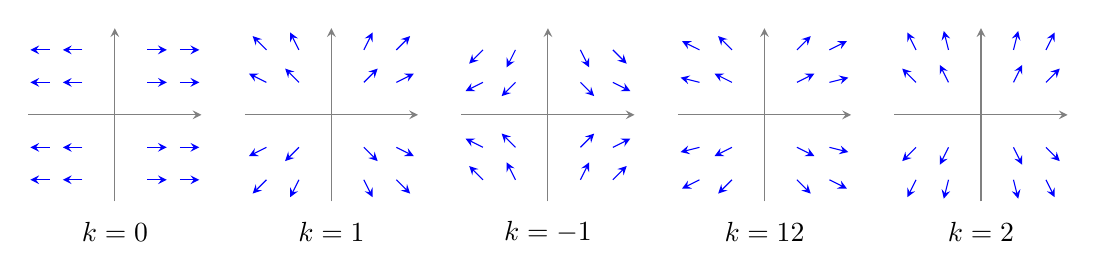
\begin{tikzpicture}[scale=.55,>=stealth]
\foreach \k/\lab/\pos in {0/0/0,1/1/5,-1/{-1}/10,.5/{1\/2}/15,2/2/20}{
\begin{scope}[xshift=\pos cm]
\draw[->,gray] (-2,0)--(2,0);\draw[->,gray](0,-2)--(0,2);
\foreach \x in {-1.5,-.75,.75,1.5}{\foreach \y in {-1.5,-.75,.75,1.5}{
\pgfmathsetmacro{\len}{sqrt(\x*\x+\k*\k*\y*\y)}
\draw[->,blue] (\x,\y)--++({.45*\x/\len},{.45*\k*\y/\len});}}
\node at (0,-2.7) {$k=\lab$};
\end{scope}}
\end{tikzpicture}
\end{center}

\prob{2.5/2}{A level set need not be one phase curve}{40}
The set $|y|=C|x|^k$ generally includes several orbits: signs of nonzero coordinates are preserved, and no nonconstant orbit can contain an equilibrium. For example, with $k=2$ a whole parabola contains its two open half-branches and the equilibrium at the origin. For $k=0$, a horizontal line consists of two open half-lines and its equilibrium on the $y$-axis. A level-set equation describes invariant sets; their maximal connected moving pieces, with equilibria separated, are the phase curves.

\prob{2.5/3}{All phase curves of a product field}{41}
For $k\ne0$, off-axis orbits are the individual quadrant branches
\[
 y=b\left(\frac{x}{a}\right)^k,\qquad x/a>0,\quad ab\ne0.
\]
There are also four coordinate half-axes and the origin. For $k>1$ branches approach zero tangent to the $x$-axis; for $0<k<1$ they are tangent to the $y$-axis; for $k=1$ they are rays. All move outward for $k>0$. For $k<0$ they are unbounded at both ends, approaching the axes asymptotically, with $|x|$ increasing and $|y|$ decreasing in forward time. For $k=0$, every $(0,b)$ is an equilibrium and the other curves are $\{(x,b):x>0\}$ and $\{(x,b):x<0\}$. In particular $y=x^2$ consists of exactly three phase curves.

\prob{2.5/4}{A very anisotropic node and saddle}{41}
For $k=.01$, $|y|=C|x|^{.01}$, equivalently $|x|=(|y|/C)^{100}$: near zero non-axial curves are almost vertical, although forward growth in $x$ is much faster than in $y$. For $k=-.01$, $|y|=C|x|^{-.01}$: the $y$-axis is stable and the $x$-axis unstable; $x$ grows on time scale one, while $y$ decays on time scale one hundred. Small $|k|$ does not turn the node or saddle into the $k=0$ equilibrium line.

\prob{2.5/5}{Inverted pendulum}{41}
Set $X=x_1+x_2$, $Y=x_1-x_2$. Then $\dot X=X$, $\dot Y=-Y$. With initial condition $(a,b)$,
\[
 x_1=a\cosh t+b\sinh t,\qquad x_2=a\sinh t+b\cosh t.
\]
The first integral is $x_1^2-x_2^2=XY=a^2-b^2$. Nonzero levels have two separate hyperbola branches. The zero level splits into the origin and four rays: $x_2=-x_1$ is stable and $x_2=x_1$ unstable. The unique velocity leading a displacement $a$ toward the upper equilibrium is $b=-a$.

\prob{2.6/1}{Four separable direction fields}{43}
Integration gives the following curves, always restricted to the domain of the displayed differential equation:
\[
\begin{array}{c|c|l}
 y'=y/x & y=Cx & x\ne0\quad\text{(rays/line segments on each half-plane)}\\
 y'=x/y & y^2-x^2=C & y\ne0\quad\text{(hyperbola branches)}\\
 y'=-y/x & xy=C & x\ne0\quad\text{(rectangular hyperbolas; also }y=0\text{)}\\
 y'=-x/y & x^2+y^2=C & y\ne0\quad\text{(upper/lower semicircles)}
\end{array}
\]
At $C=0$ in the second equation the lines $y=\pm x$ are split at the excluded origin. In the fourth equation $C>0$; the origin is not in the equation's domain. Vertical tangencies of the implicit curves require switching independent variable rather than pretending $y(x)$ stays differentiable there.

\prob{2.6/2}{Powers and trigonometric examples}{43}
For $y'=kx^\alpha y^\beta$, on a real smooth branch with $y\ne0$ define
\[
 F_\gamma(s)=\begin{cases}s^{1-\gamma}/(1-\gamma),&\gamma\ne1,\\\log|s|,&\gamma=1.\end{cases}
\]
Then the curves are $F_\beta(y)=kF_{-\alpha}(x)+C$. This includes the logarithmic cases $\alpha=-1$ or $\beta=1$. If $y=0$ belongs to the domain and the right-hand side vanishes there, add that solution; if the right-hand side is not locally Lipschitz there, additional glued solutions may occur. For $k=0$ all admissible horizontal lines are solutions. Arbitrary real powers should normally be read on $x>0,y>0$, unless a different real branch is specified.

For the remaining equations,
\[
 \frac{\mathrm dy}{\mathrm dx}=\frac{\sin y}{\sin x}
 \quad\Longrightarrow\quad
 \log|\tan(y/2)|=\log|\tan(x/2)|+C,
\]
where separation is valid, together with $y=m\pi$; the domain excludes $x=n\pi$. Equivalently $\tan(y/2)=A\tan(x/2)$ on each admissible chart. For
\[
 \frac{\mathrm dy}{\mathrm dx}=\frac{\sin x}{\sin y},\qquad
 \cos y-\cos x=C,
\]
restrict to $\sin y\ne0$. These implicit level sets describe the requested sketches; their repeated cells follow from $2\pi$-periodicity. Each connected graph branch is taken separately.

\prob{2.6/3}{Pendulum phase portrait}{43}
For $\dot x=y$, $\dot y=-\sin x$, the energy
\[
 E=\frac{y^2}{2}+1-\cos x
\]
is constant. At $E=0$ are the centers $(2m\pi,0)$. For $0<E<2$, closed ovals surround each center, traversed clockwise. At $E=2$ the saddles $((2m+1)\pi,0)$ and the separatrix branches $y=\pm2|\cos(x/2)|$ are distinct orbits. For $E>2$, $y=\pm\sqrt{2(E-1+\cos x)}$ are rotations: the upper branches run right, the lower left. They are not closed on the covering plane, but are closed on the cylinder $x\bmod2\pi$.
\begin{center}
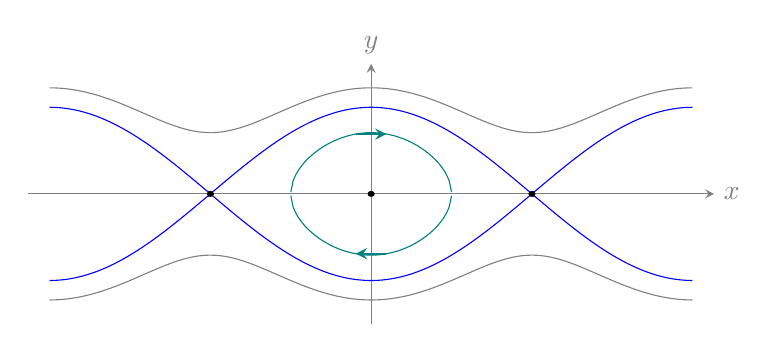
\begin{tikzpicture}[xscale=.65,yscale=.55,>=stealth]
\draw[->,gray](-6.7,0)--(6.7,0)node[right]{$x$};\draw[->,gray](0,-3)--(0,3)node[above]{$y$};
\foreach \sgn in {-1,1}{
\draw[blue,domain=-6.28:6.28,samples=140]plot(\x,{\sgn*2*abs(cos(\x*180/pi/2))});
\draw[gray,domain=-6.28:6.28,samples=140]plot(\x,{\sgn*sqrt(2*(2+cos(\x*180/pi)))});
\draw[teal,domain=-1.57:1.57,samples=70]plot(\x,{\sgn*sqrt(max(0,2*cos(\x*180/pi)))});}
\fill(0,0)circle(2pt);\foreach \x in {-3.1416,3.1416}{\fill(\x,0)circle(2pt);}
\draw[->,teal,thick](-.3,1.38)--(.3,1.38);\draw[->,teal,thick](.3,-1.38)--(-.3,-1.38);
\end{tikzpicture}
\end{center}

\prob{2.7/1}{Divergence of the Lotka--Volterra period}{44}
Assume $a,b,k,l>0$, and initial states strictly inside the positive quadrant. Put $x_*=l/b$, $y_*=k/a$, $u=\log(x/x_*)$, $v=\log(y/y_*)$. Then
\[
 \dot u=k(1-e^v),\quad \dot v=l(e^u-1),\qquad
 E=l(e^u-u-1)+k(e^v-v-1)
\]
is conserved. As $(x,y)\to(0,0)$, $E\to\infty$. At the leftmost point of an energy oval, $v=0$ and $u=u_-<0$, where $l(e^{u_-}-u_--1)=E$, so $u_-=-E/l+O(1)$. During the arc from this point to $u=0$ in $v<0$, $\dot u\le k$. Hence
\[
 T(E)\ge\frac{-u_-}{k}=\frac{E}{kl}+O(1)\longrightarrow\infty.
\]
States on the axes themselves are not periodic, so the limiting statement concerns interior states.

\prob{2.7/2}{Logarithmic divergence near an axis}{44}
At $(x_*,\varepsilon)$, the energy above satisfies $E=k\log(1/\varepsilon)+O(1)$. The preceding estimate gives $T\ge cE$ for large $E$. We prove a matching upper bound, which makes ``logarithmically'' precise as $T=\Theta(\log(1/\varepsilon))$.

Fix $\delta>0$. On an energy oval, $u,v$ range between $-O(E)$ and $O(\log E)$. In each quadrant, outside the strips $|u|<\delta$ and $|v|<\delta$, both $|\dot u|$ and $|\dot v|$ are bounded below by a positive constant depending only on the parameters and $\delta$. Both coordinates are monotone on each quadrant arc. Its time there is at most a constant times its coordinate range, hence $O(E)$. Inside $|u|<\delta$, large energy forces $|v|>\delta$, so $|\dot u|$ is bounded below and passage across each such strip takes $O(1)$. Similarly passage through $|v|<\delta$ takes $O(1)$ using $\dot v$. A quadrant arc meets each strip at most once. Adding the finitely many pieces proves $T\le CE$. This establishes upper and lower logarithmic bounds without claiming an unproved exact asymptotic coefficient.

\prob{2.7/3}{Birth and collision of limit cycles}{46--47}
Write $s=r^2$. Positive-radius cycles satisfy $s^2-s+c=0$, hence
\[
 s_\pm=\frac{1\pm\sqrt{1-4c}}2.
\]
At a positive root the derivative of $F(r)=cr-r^3+r^5$ is $F'(r)=2s(2s-1)$. Thus $r_-=\sqrt{s_-}$ is attracting and $r_+=\sqrt{s_+}$ repelling whenever both exist.
\begin{center}\begin{tabular}{p{.15\linewidth}p{.72\linewidth}}\toprule
Parameter & Behavior\\\midrule
$c<0$ & Origin attracting; one repelling cycle $r_+>1$.\\
$c=0$ & Origin still attracting ($\dot r\sim-r^3$); repelling cycle $r=1$.\\
$0<c<1/4$ & Origin repelling; attracting inner and repelling outer cycles.\\
$c=1/4$ & Double cycle $r=1/\sqrt2$, attracting from inside and repelling from outside.\\
$c>1/4$ & No cycles; every $r>0$ increases.\\\bottomrule
\end{tabular}\end{center}
As $c\downarrow0$ through positive values, $r_-\sim\sqrt c$. At $c=1/4$ the cycles merge; their squared-radius separation is $\sqrt{1-4c}$. Each cycle has period $2\pi$, since $\dot\varphi=1$. The origin is an equilibrium of the associated smooth Cartesian system, despite the polar angle being undefined there.

\section{Linear equations (\texorpdfstring{$\S3$}{Section 3})}
\review{On an interval, all solutions of $y'=f(x)y$ are $Ce^{\int_{x_0}^x f}$, so the solution space is one-dimensional. For $T$-periodic $f$, set $\lambda=e^{\int_0^T f}>0$. Writing $x=nT+s$, $0\le s<T$, gives $y(x)=\lambda^n y(s)$. For a nonzero solution, $|y(s)|$ has positive minimum and finite maximum on $[0,T]$, proving decay for $\lambda<1$, divergence in absolute value for $\lambda>1$, and periodicity for $\lambda=1$. A negative solution diverges to $-\infty$, not $+\infty$.}

\prob{3.2/1}{From a multiplier to stability of a cycle}{51}
In coordinates near the cycle write $Y'=a(X,Y)$, $a(X,0)=0$, with period $T$ in $X$. Let $P(\eta)$ be the return map. Differentiating the solution with respect to its initial transverse coordinate gives $z'=a_Y(X,0)z$, $z(0)=1$, so
\[
 P(0)=0,\qquad P'(0)=\lambda=\exp\int_0^T a_Y(X,0)\dd X.
\]
If $\lambda<1$, choose $q$ between $\lambda$ and one. Near zero the mean-value theorem gives $|P(\eta)|\le q|\eta|$, and iterates converge to zero. Smooth dependence over the compact time interval $[0,T]$ bounds intermediate deviations by a constant times the section deviation, so the full phase curve spirals toward the cycle. If $\lambda>1$, $|P(\eta)|\ge q|\eta|$ for some $q>1$ while it remains nearby, so nonzero deviations eventually leave a fixed neighborhood; the inverse return map is contracting. This is repulsion, or outward spiraling. At $\lambda=1$ linearization alone decides neither case.

\prob{3.2/2}{A cycle with alternating radial attraction and repulsion}{51}
Since $\dot\varphi=1$, use $\varphi$ as time in $\dot r=(r^2-1)(2r\cos\varphi-1)$. At $r=1$ the transverse linear coefficient is
\[
 f(\varphi)=2(2\cos\varphi-1)=4\cos\varphi-2.
\]
Therefore $\lambda=\exp\int_0^{2\pi}f\dd\varphi=e^{-4\pi}<1$, and the cycle is asymptotically stable. Instantaneous radial expansion on some arcs does not outweigh the contraction over a full revolution.

\review{For a nonnegative delta-shaped sequence $h_N$ supported in $[-\varepsilon_N,\varepsilon_N]$, with integral one and $\varepsilon_N\to0$, continuity gives
$|\int h_N(x)g(x)\dd x-g(0)|\le\sup_{|x|\le\varepsilon_N}|g(x)-g(0)|\to0$.
This proves the embedded claim on p.~54. No ordinary function with integral one and support at a single point exists.}

\prob{3.4/1}{A rectangular impulse and its limit}{56}
Let $a_N=1-1/(2N)$, $b_N=1+1/(2N)$, and let $h_N=N$ on $(a_N,b_N)$ and zero elsewhere. The integrating-factor formula gives
\[
 y_N(x)=\begin{cases}
 0,&x\le a_N,\\
 N(e^{x-a_N}-1),&a_N\le x\le b_N,\\
 N(e^{x-a_N}-e^{x-b_N}),&x\ge b_N.
 \end{cases}
\]
This is continuous and piecewise differentiable, and solves the equation almost everywhere; the discontinuous forcing prevents a classical derivative at the two switching points. Pointwise,
\[
 y_N(x)\longrightarrow
 \begin{cases}0,&x<1,\\1/2,&x=1,\\e^{x-1},&x>1.\end{cases}
\]
At $x=1$, use $N(e^{1/(2N)}-1)\to1/2$. Convergence is locally uniform away from one, not across the jump. The distributional limit is the causal Green function $H(x-1)e^{x-1}$; its value at the single jump point is immaterial distributionally and depends on the regularization.

\prob{3.5/1}{Periodic forcing with damping}{56--57}
A particular solution of $y'=-y+\sin x$ is
\[
 y_p(x)=\tfrac12(\sin x-\cos x),\qquad y(x)=y_p(x)+Ce^{-x}.
\]
Only $C=0$ is periodic, since a nonzero $Ce^{-x}$ cannot have period $2\pi$. Every solution converges exponentially to $y_p$ as $x\to\infty$. The multiplier is $e^{-2\pi}$.
\review{For general periodic $f,g$, put $A(x)=e^{\int_0^x f}$. Then $y(T)=A(T)y(0)+A(T)\int_0^T A(s)^{-1}g(s)\dd s$, an affine map as claimed on p.~56. If $A(T)\ne1$ it has exactly one fixed point, giving the unique periodic solution. If $A(T)=1$, it has either no fixed points or every point is fixed, according to whether the added constant is nonzero or zero.}

\prob{3.5/2}{The inhomogeneous variational equation}{57}
Differentiate $\partial_t\phi(t,\varepsilon)=v(t,\phi(t,\varepsilon);\varepsilon)$ at $\varepsilon=0$. Smoothness permits interchanging derivatives and applying the chain rule:
\[
 \dot\psi=v_x(t,\phi_0(t);0)\psi+v_\varepsilon(t,\phi_0(t);0).
\]
Thus $f=v_x$ and $g=v_\varepsilon$ along the reference solution. If the initial value depends on $\varepsilon$, the initial condition is $\psi(t_0)=\partial_\varepsilon\phi(t_0,0)$; if it is fixed, this is zero. For systems $f$ becomes the Jacobian matrix.

\section{Phase flows (\texorpdfstring{$\S4$}{Section 4})}
\prob{4.1/1}{Which maps are transformations?}{57}
A transformation here is a bijection of the specified set onto itself. The exponential misses the nonpositive real numbers, $x^3$ is a bijection of $\R$ with inverse $\sqrt[3]{x}$, and $z^2$ is not injective on $\C$ since $z$ and $-z$ have the same square. Only the second is a transformation. Smoothness of its inverse is not yet required.

\prob{4.1/2}{Noncommuting transformations}{58}
On $\R$ take $f(x)=x+1$, $g(x)=2x$. Then $(fg)(x)=2x+1$ while $(gf)(x)=2x+2$, so $fg\ne gf$.

\prob{4.1/3}{Three reflections}{58}
No. The three vertex-axis reflections of an equilateral triangle do not include the identity, although the square of each is the identity. The product of two distinct reflections is a rotation by $\pm2\pi/3$, also absent. The six-element group generated by them does include these maps.

\prob{4.1/4}{Triangle isometries and tetrahedron rotations}{58}
An equilateral triangle's three rotations (including the identity) and three reflections give six isometries. A regular tetrahedron has the identity, eight rotations by $\pm2\pi/3$ about its four vertex--opposite-face axes, and three half-turns about opposite-edge-midpoint axes: twelve in total. Equivalently these realize all even permutations of its four vertices.

\prob{4.1/5}{The additive group of real numbers}{58}
Addition is associative, zero is an identity, and each $a$ has inverse $-a$; closure is automatic. To fit the book's transformation-group definition, use $T_a(x)=x+a$. Then $T_aT_b=T_{a+b}$, $T_a^{-1}=T_{-a}$, and the representation is faithful.

\prob{4.1/6}{Permutations of coordinate axes by cube isometries}{59}
Every permutation $\sigma\in S_3$ is realized by the orthogonal permutation matrix $e_i\mapsto e_{\sigma(i)}$, which preserves $\max(|x|,|y|,|z|)$. Thus all six permutations occur. Even if only rotations are allowed, signs can be chosen to make the signed permutation matrix have determinant $+1$ without changing its action on the unoriented axes.

\prob{4.1/7}{Action on matrices}{59}
Under the coordinate change $y=gx$, an operator $x\mapsto Mx$ becomes $y\mapsto gMg^{-1}y$. Hence $T_g(M)=gMg^{-1}$. Moreover $T_gT_h=T_{gh}$ and $T_{g^{-1}}=T_g^{-1}$. If one instead describes a change of basis by giving the new basis in old coordinates, the inverse convention produces $g^{-1}Mg$; the distinction is purely the meaning assigned to $g$.

\prob{4.1/8}{Rotation orbits}{59}
Rotations preserve distance from zero and act transitively on every circle of fixed positive radius. The orbits are therefore the origin and all circles centered at the origin.

\prob{4.1/9}{Orbits partition a set}{59}
If $z=gx=hy$ belongs to both $Gx$ and $Gy$, then $y=h^{-1}gx$, so every $ky$ lies in $Gx$. This gives $Gy\subseteq Gx$; reversing the argument gives equality. Otherwise the two orbits are disjoint.

\prob{4.1/10}{Unordered pairs of tetrahedron edges}{59}
For two distinct edges there are two invariant possibilities: they share a vertex, or they are opposite. Vertex permutations act transitively on each type, so there are two orbits (of sizes twelve and three). If ``pairs'' were to allow a repeated edge, the six double-edge pairs form a third orbit. The standard interpretation is a two-element subset, giving two.

\prob{4.1/11}{Six distinct colors on a cube}{59}
There are $6!$ labelings using every color once. A rotation is determined by the image of one face (six choices) and then one adjacent face (four choices), so the rotation group has order twenty-four. Its action on distinct-color labelings is free: a color-preserving rotation fixes all faces and is the identity. Every orbit thus has size twenty-four, giving $6!/24=30$ colorings up to rotation.

\prob{4.3/1}{Diffeomorphisms of the real line}{61}
Only $x$ and $-x$ are diffeomorphisms of $\R$ onto itself. The square is not injective, the cube has an inverse not differentiable at zero, and $\arctan x$ is not onto $\R$. The last map is a diffeomorphism onto $(-\pi/2,\pi/2)$, which is a different codomain.

\prob{4.3/2}{Must a linear flow split into one-dimensional factors?}{63}
No, over $\R$. A nontrivial rotation flow has no common invariant real line, whereas a direct product would have two. A shear $g^t(x,y)=(x+ty,y)$ supplies another obstruction: its infinitesimal matrix $\left(\begin{smallmatrix}0&1\\0&0\end{smallmatrix}\right)$ is not diagonalizable. A linear splitting would diagonalize this matrix, an impossibility.

\prob{4.4/1}{Generators of three line flows}{63}
Differentiate at $t=0$: $x+t$ gives $v(x)=1$, $e^tx$ gives $v(x)=x$, and $e^{-t}x$ gives $v(x)=-x$.

\prob{4.4/2}{Zeros of the generator are fixed points}{63}
If $v(a)=0$, the constant curve at $a$ solves $\dot x=v(x)$. The orbit $g^ta$ solves the same initial-value problem, so uniqueness yields $g^ta=a$. Conversely differentiating a fixed orbit gives $v(a)=0$.

\prob{4.4/3}{Every solution is an orbit of the given flow}{64}
For a solution with $\phi(0)=x_0$, the curve $g^tx_0$ satisfies the same equation and initial condition. Uniqueness identifies them on the entire domain of $\phi$. More generally, $\phi(t)=g^{t-t_0}\phi(t_0)$.

\prob{4.4/4}{Four explicit flows}{64}
Solving with initial value $x$ at time zero gives
\[
\begin{array}{c|c}
 \dot x=0 & g^t(x)=x\\
 \dot x=1 & g^t(x)=x+t\\
 \dot x=x-1 & g^t(x)=1+(x-1)e^t\\
 \dot x=\sin x,\quad0<x<\pi & g^t(x)=2\arctan(e^t\tan(x/2)).
\end{array}
\]
For the last formula integrate $\dd x/\sin x=\dd t$; the chosen branch stays in $(0,\pi)$ for every finite $t$. Each formula has inverse $g^{-t}$ and satisfies the group law.

\prob{4.4/5}{Three planar flows}{64--65}
For initial state $(x,y)$, successive integration gives
\[
\begin{array}{c|c}
 (\dot x,\dot y)=(y,0)&g^t(x,y)=(x+ty,y)\\
 (\dot x,\dot y)=(y,1)&g^t(x,y)=(x+ty+t^2/2,y+t)\\
 (\dot x,\dot y)=(\sin y,0)&g^t(x,y)=(x+t\sin y,y).
\end{array}
\]
Differentiating verifies the equations and setting $t=0$ verifies the initial states. These polynomial/trigonometric formulas exist for every real $t$.

\prob{4.4/6}{At most linear growth implies completeness}{65}
Suppose $|v(x)|\le a+b|x|$ with $a,b\ge0$. Gronwall gives, on any finite interval measured from zero,
\[
 |x(t)|\le (|x(0)|+a/b)e^{b|t|}-a/b\quad(b>0),
\]
and $|x(t)|\le|x(0)|+a|t|$ if $b=0$. The same bound holds backward by reversing time. Thus no solution escapes to infinity in finite time. A solution confined to a compact interval can be extended by local existence, so every maximal solution is global. Smooth dependence and uniqueness give smooth maps $g^t$, the group law, and inverse $g^{-t}$; hence a one-parameter diffeomorphism group.

\prob{4.4/7}{The field $e^x\sin x$}{65}
Yes. Every $n\pi$ is an equilibrium, and uniqueness confines any other solution to its initial interval $(n\pi,(n+1)\pi)$. Its closure is compact and the field is smooth there, so no finite-time escape occurs. A zero of a smooth scalar field cannot be reached in finite time either. All solutions are complete even though the field has no global linear-growth bound.

\prob{4.4/8}{Translation on a polynomial space}{66}
Let $P_{<n}$ be the vector space of polynomials of degree less than $n$. The map $(g^tp)(x)=p(x+t)$ is linear in $p$, preserves this space, satisfies $g^sg^t=g^{s+t}$, and has inverse $g^{-t}$. Its coefficients depend polynomially on $t$, so the flow is smooth. Its generator is $Dp=p'$; in the basis $1,x,\ldots,x^{n-1}$ this sends $x^j$ to $jx^{j-1}$. Since $D^n=0$, the flow is the finite sum $e^{tD}=\sum_{j=0}^{n-1}t^jD^j/j!$.

\section{Changes of variables and fields (\texorpdfstring{$\S5$}{Section 5})}
\prob{5.1/1}{Independence of the curve representing a tangent vector}{67}
If $\phi(0)=\psi(0)=x$ and $\phi'(0)=\psi'(0)=v$, then $\phi(t)-\psi(t)=o(|t|)$. Smoothness of $f$ gives a local Lipschitz bound, so $f(\phi(t))-f(\psi(t))=o(|t|)$. Their derivatives at zero therefore agree. Equivalently, the chain rule gives $(f\circ\phi)'(0)=Df_xv$ for either curve.

\prob{5.1/2}{A unit vector under squaring}{67}
For $f(x)=x^2$, $Df_a(v)=2av$. A positive unit vector has component one, so the image has component $2a$, attached at $a^2$. It is negative when $a<0$ and zero when $a=0$.

\prob{5.1/3}{Motions along different axes with the same velocity}{67}
Yes, but only with zero common velocity, since the two coordinate-axis tangent lines intersect only in zero. The curves $\phi(t)=(t^2,0)$ and $\psi(t)=(0,t^2)$ both leave the origin with zero derivative while moving on different axes.

\prob{5.1/4}{Linearity of the derivative}{68}
Differentiability means $f(x+h)=f(x)+Ah+o(|h|)$ for a linear map $A=Df_x$. Applying this to a curve with $h=tv+o(t)$ gives $f_{*x}v=Av$. Hence $f_{*x}(av+bw)=af_{*x}v+bf_{*x}w$. In coordinates $(f_*v)_i=\sum_j(\partial f_i/\partial x_j)v_j$.

\prob{5.1/5}{Derivative of a circle parametrization}{68}
For $f(x)=(\sin x,\cos x)$ and $v=10\partial_x$ at $\alpha$,
\[
 f_{*\alpha}v=(10\cos\alpha,-10\sin\alpha),
\]
attached at $(\sin\alpha,\cos\alpha)$. Its norm is ten and it is tangent to the circle.

\prob{5.1/6}{Critical points and values of the cusp map}{68}
For $f(x_1,x_2)=(x_1^3+x_1x_2,x_2)$,
\[
 Df=\begin{pmatrix}3x_1^2+x_2&x_1\\0&1\end{pmatrix}.
\]
Its determinant vanishes on $x_2=-3x_1^2$. Parametrizing that parabola by $s=x_1$ gives critical values $(y_1,y_2)=(-2s^3,-3s^2)$, hence
\[
 \frac{y_1^2}{4}+\frac{y_2^3}{27}=0.
\]
Conversely every real point on this semicubical parabola has such a parameter, so the equation describes the entire critical-value set.

\prob{5.1/7}{A diffeomorphism induces tangent-space isomorphisms}{70}
Apply the chain rule to $f^{-1}\circ f=\mathrm{id}$ and $f\circ f^{-1}=\mathrm{id}$. It gives $D(f^{-1})_{f(x)}Df_x=I$ and $Df_xD(f^{-1})_{f(x)}=I$. Thus $Df_x$ is an isomorphism with the indicated inverse. In terms of curves, applying $f^{-1}$ recovers the original tangent-vector class.

\prob{5.1/8}{Invertible derivatives do not imply a global diffeomorphism}{70}
The map $f(u,v)=(e^u\cos v,e^u\sin v)$ from $\R^2$ onto $\R^2\setminus\{0\}$ has Jacobian determinant $e^{2u}>0$, but $f(u,v+2\pi)=f(u,v)$, so it is not injective. The inverse-function theorem yields local inverses, not a global one.

\prob{5.2/1}{Pushforward by dilation}{71}
For $g(x)=2x$ and $v=\partial_x$, the field at $y=g(x)$ is $Dg_xv(x)=2$. Thus $g_*v=2\partial_y$.

\prob{5.2/2}{Pushforward of the Euler field by the exponential}{71}
For $v=x\partial_x$ and the diffeomorphism $y=e^x$ from $\R$ onto $(0,\infty)$, the chain rule gives
\[
 g_*v=xe^x\partial_y=y\log y\,\partial_y.
\]
The coefficient must be expressed at the image point, so substitute $x=\log y$ after multiplying by $g'(x)=e^x$. The equilibrium at $x=0$ becomes the equilibrium at $y=1$.
\prob{5.2/3}{Linear invariance of the Euler field}{71}
For an invertible linear map $g(x)=Ax$ and $v(x)=x$, one has $(g_*v)(y)=A(A^{-1}y)=y$. Thus rotations, hyperbolic rotations, and all invertible linear transformations preserve the Euler field. Invertibility is required because the question concerns diffeomorphisms.

\prob{5.2/4}{Phase curves versus time-parametrized trajectories}{72}
If $g_*v=w$ and $x'=v(x)$, then $(g\circ x)'=Dg_xv(x)=w(g(x))$, so phase curves map to phase curves with time preserved. The converse fails: the identity maps all phase curves of $x\partial_x$ onto those of $2x\partial_x$ (the two open rays and zero), but does not map the first field to the second. Their speeds differ by two.

\prob{5.3/1}{Polar solution of the oscillator}{72}
For $r>0$, $\dot r=(x_1\dot x_1+x_2\dot x_2)/r=0$ and $\dot\theta=(x_1\dot x_2-x_2\dot x_1)/r^2=-1$. Thus
\[
 x_1=r_0\cos(\theta_0-t),\qquad x_2=r_0\sin(\theta_0-t).
\]
Add the equilibrium at zero, where polar coordinates are not a chart.

\prob{5.3/2}{A stable circular limit cycle}{72--73}
For the displayed system, polar coordinates give $\dot r=r(1-r^2)$, $\dot\theta=-1$. For $r_0>0$,
\[
 r(t)=\left[1+(r_0^{-2}-1)e^{-2t}\right]^{-1/2},\qquad
 \theta(t)=\theta_0-t,
\]
on the maximal interval where the bracket is positive. The origin is repelling, the unit circle is a clockwise periodic orbit of period $2\pi$, and every other nonzero trajectory spirals toward it in forward time. If $r_0<1$ the solution is global and tends to zero backward; if $r_0>1$ it blows up at a finite negative time. Thus forward attraction does not imply a global two-sided flow on the plane.

\prob{5.4/1}{A direction field without a nonvanishing vector representative}{74}
On the punctured plane write a point as $(r,\theta)$ and prescribe the unoriented line
\[
 L_{r,\theta}=\operatorname{span}(\cos(\theta/2),\sin(\theta/2)).
\]
It is single-valued and smooth as a line field because increasing $\theta$ by $2\pi$ changes the vector's sign but not its span. A nonvanishing continuous representative on the unit circle would be $a(\theta)(\cos(\theta/2),\sin(\theta/2))$, with $a$ continuous and nonzero. Periodicity forces $a(2\pi)=-a(0)$, contradicting the intermediate-value theorem. The field therefore cannot be represented by a nowhere-zero vector field. Allowing the zero field would make the question vacuous: zero does not determine a direction.

\prob{5.4/2}{Separating a homogeneous equation}{74}
For $\mathrm dx/\mathrm dt=(x^2-t^2)/(x^2+t^2)$, use $u=x/t$ on either half-plane $t\ne0$. Then
\[
 u+t\frac{\mathrm du}{\mathrm dt}=\frac{u^2-1}{u^2+1},\qquad
 \frac{u^2+1}{-u^3+u^2-u-1}\dd u=\frac{\dd t}{t}.
\]
This separates the variables. Roots of $-u^3+u^2-u-1=0$ yield the straight solutions $x=ut$ lost by division. The original equation is undefined only at $(0,0)$; use the complementary chart $t/x$ where needed. Alternatively, polar coordinates $t=r\cos\theta,x=r\sin\theta$ give
\[
 \frac{\dd r}{r}=\frac{\cos\theta-\sin\theta\cos2\theta}{-\sin\theta-\cos\theta\cos2\theta}\dd\theta,
\]
where the denominator is nonzero; its zero directions are again handled separately.

\prob{5.4/3}{Straightening $x'=x-1$ globally}{74}
The map $F(t,x)=(t,a)$, $a=e^{-t}(x-1)$, is a global diffeomorphism with inverse $(t,a)\mapsto(t,1+ae^t)$. Along a solution, $a'=e^{-t}(x'-x+1)=0$, so the integral curves become the parallel lines $a=\text{constant}$.

\prob{5.4/4}{A plane direction field that cannot be straightened globally}{74--75}
Consider the smooth nowhere-zero vector field $V(t,x)=(\cos x,\sin x)$ on the entire plane. The lines $x=0$ and $x=\pi$ are distinct leaves. In the strip $0<x<\pi$ the other leaves satisfy
\[
 \frac{\dd t}{\dd x}=\cot x,\qquad t=\log(\sin x)+C.
\]
Their two ends approach the two boundary leaves as $t\to-\infty$. More precisely, any saturated open neighborhoods of the two boundary leaves intersect: take small neighborhoods of $(0,0)$ and $(0,\pi)$. For $C$ sufficiently large, the leaf $t=\log(\sin x)+C$ crosses both at $t=0$, since $\sin x=e^{-C}$ has roots close to both endpoints. Thus the two leaves cannot be separated in the quotient space of leaves. A foliation by parallel lines has leaf space $\R$, which is Hausdorff. A diffeomorphism mapping leaves to leaves induces a homeomorphism of leaf spaces, so no such global straightening exists.

\prob{5.4/5}{Global straightening of $x'=x^2$}{75}
Despite finite-time explosion, the answer for its direction field in the $(t,x)$-plane is yes. Rescale its vector representative to
\[
 W(t,x)=\frac{(1,x^2)}{1+x^2}.
\]
Both components are bounded, so $W$ is complete. The function $s=t+x$ satisfies $W(s)=1$. Therefore every orbit meets the transversal $\Gamma=\{(-a,a):a\in\R\}$ exactly once: following the complete flow for time $-s$ reaches $\Gamma$. If $\Phi_W$ is that flow, then
\[
 (s,a)\longmapsto\Phi_W^s(-a,a)
\]
is a global smooth bijection with smooth inverse, by the flow property and transversality. It takes horizontal lines $a=\text{constant}$ to the desired integral curves.

For an explicit expression for the second coordinate of the inverse, one may use
\[
 a(t,x)=\frac{2x}{1-tx+\sqrt{(1-tx)^2+4x^2}}.
\]
The denominator is strictly positive (also at $x=0$), and this is smooth. For $x\ne0$ it is obtained by equating the first integral $t+1/x$ to its value $-a+1/a$ on $\Gamma$; it extends with $a(t,0)=0$. Thus $F(t,x)=(t+x,a(t,x))$ is the promised explicit diffeomorphism. This straightens a direction field, not the original time-parametrized incomplete flow.

\prob{5.5/1}{Conjugation preserves the flow laws}{75}
For $h^t=fg^tf^{-1}$,
\[
 h^sh^t=fg^sf^{-1}fg^tf^{-1}=fg^{s+t}f^{-1}=h^{s+t},
 \quad h^0=\mathrm{id},\quad(h^t)^{-1}=h^{-t}.
\]
Each map is a diffeomorphism and the dependence on $(t,y)$ is smooth. Hence this is a one-parameter diffeomorphism group.

\prob{5.5/2}{Circular and hyperbolic rotations are not conjugate}{76}
Every nonzero orbit of a circular rotation flow is compact and periodic. Every nonzero orbit of a hyperbolic rotation $(x,y)\mapsto(e^tx,e^{-t}y)$ is nonperiodic and noncompact. A conjugacy preserves periodicity (indeed the exact periods), so these flows cannot be conjugate. Also the circular flow has $g^{2\pi}=\mathrm{id}$, whereas the hyperbolic flow does not.

\prob{5.5/3}{Classifying five scalar vector fields}{76}
Write
\[
 v_1=\sin x,\quad v_2=2\sin x,\quad v_3=\sin^2x,\quad
 v_4=\sin2x,\quad v_5=2\sin x+\sin^2x.
\]
For a diffeomorphism $h$ satisfying $h'v=w\circ h$, zeros correspond and differentiation at a zero $a$ gives $v'(a)=w'(h(a))$. The zero derivatives of $v_1$ alternate $\pm1$, those of $v_2,v_4,v_5$ alternate $\pm2$, and those of $v_3$ are zero. Thus the only possible equivalences between different members are within $\{v_2,v_4,v_5\}$. The map $h(x)=x/2$ takes $v_2$ to $v_4$ directly.

Here is a full existence argument for the harder equivalence of $v_2$ and $v_5$. Both have exactly the simple zeros $n\pi$, the same sign on each interval between zeros, and matching derivatives there. We use two elementary constructions.

\emph{Local construction at a simple zero.} If $v(a)=0$, $v'(a)=\lambda\ne0$, write $z=x-a$. The function
\[
 q_v(x)=z\exp\left(\int_0^z\left[\frac{\lambda}{v(a+s)}-\frac1s\right]\dd s\right)
\]
is smooth near $a$, has derivative one at $a$, and satisfies $q_v'v=\lambda q_v$. The integrand extends smoothly at zero: write $v(a+s)=s(\lambda+s b(s))$. Thus matching fields with the same $\lambda$ are locally conjugate by $q_w(h(x))=c q_v(x)$ for any $c>0$. Every increasing conjugacy on one side near the zero has exactly this form, because the ratio of the two linearizing coordinates is constant along the scalar equation.

\emph{Extension across a zero-free interval.} On $(n\pi,(n+1)\pi)$ the time coordinates $\int\dd x/v(x)$ and $\int\dd y/w(y)$ are monotone onto $\R$; the logarithmic divergences at the endpoints ensure this. Equating them up to an additive constant therefore defines an increasing diffeomorphism of that interval. Starting with a local conjugacy near zero, this extends uniquely through $(0,\pi)$ and approaches $\pi$. Near $\pi$ it has the local form just proved, with a positive constant $c$, so it extends smoothly across $\pi$ with nonzero derivative. Continue inductively in both directions. Since the zeros have no finite accumulation point, this yields a smooth increasing diffeomorphism $h:\R\to\R$ mapping each $n\pi$ to itself and satisfying $h'v_2=v_5\circ h$ everywhere. It is onto because it maps every consecutive interval onto itself.

The equivalence classes among the five displayed fields are therefore $\{v_1\}$, $\{v_3\}$, and $\{v_2,v_4,v_5\}$. No periodicity condition is imposed on $h$; the proof is for the line as requested, not a prescribed conjugacy on a fixed circle.

\section{Symmetries (\texorpdfstring{$\S6$}{Section 6})}
\prob{6.1/1}{Preserving phase curves need not preserve a field}{76}
For $v=\partial_x$ on $\R$, the diffeomorphism $h(x)=2x$ preserves its sole maximal phase curve, the whole line, but $h_*v=2\partial_x\ne v$. Preserving the paths does not preserve speed. The same example on the plane, with $v=\partial_x$ and $h(x,y)=(2x,y)$, preserves each horizontal phase line.

\prob{6.1/2}{Preserving integral curves preserves a direction field}{77}
At each point, the prescribed line is the tangent line to the integral curve through that point. The derivative of a diffeomorphism taking integral curves to integral curves takes their tangent lines to their tangent lines. It therefore preserves the direction field. Speed and orientation along a line are irrelevant here.
\review{The identity is a symmetry; if $f_*v=v$ and $g_*v=v$, then $(f\circ g)_*v=f_*(g_*v)=v$; applying the inverse pushforward shows $f^{-1}$ is a symmetry. The same proof applies to direction fields, answering the embedded group question on p.~77.}

\prob{6.1/3}{All global symmetries of the Euler field}{77}
A symmetry $h:\R^2\to\R^2$ of $v(x)=x$ fixes its unique zero and commutes with its flow, so $h(0)=0$ and $h(e^tx)=e^th(x)$. For $s>0$ this gives $h(sx)=sh(x)$. Differentiability at zero now forces
\[
 h(x)=\lim_{s\downarrow0}\frac{h(sx)-h(0)}s=Dh_0x.
\]
Thus $h$ is an invertible linear map. Conversely every such map preserves the Euler field. The full group is $GL(2,\R)$. The inclusion of the origin and differentiability there are essential; on the punctured plane there are nonlinear homogeneous symmetries.

\prob{6.2/1}{Reducing dimension using a one-parameter symmetry}{79}
Work locally where the symmetry generator is nonzero. Straighten its flow to translation in a coordinate $u$, with transverse coordinates $z\in\R^{n-1}$. An invariant line field can locally be represented by a nonvanishing vector whose components depend only on $z$:
\[
 \dot u=A(z),\qquad \dot z=B(z).
\]
To see this, normalize one nonzero component of any representative to one; translation invariance of the line makes all ratios of components independent of $u$. Where $B\ne0$, solve the reduced $(n-1)$-dimensional direction field spanned by $B$. Choose its parametrization so that $\dot z=B(z)$ and then recover $u$ by the quadrature $u=u_0+\int A(z(t))\dd t$. If $B(z_0)=0$, the leaf there is a symmetry orbit $z=z_0$, and the remaining equation is one-dimensional. The reduction is local; a global orbit space need not be a manifold, and fixed points of the symmetry require separate treatment.

\prob{6.3/1}{Three homogeneous equations}{79}
Each right-hand side is unchanged by $(x,y)\mapsto(\lambda x,\lambda y)$ for $\lambda>0$:
\[
 \frac{\lambda y}{\lambda x}=\frac yx,\quad
 \frac{\lambda x}{\lambda y}=\frac xy,\quad
 \log(\lambda x)-\log(\lambda y)=\log x-\log y.
\]
Thus all three are homogeneous on their stated domains. In the logarithmic example both coordinates are positive.

\prob{6.3/2}{A homogeneous Riccati-type equation}{80}
Set $y=xv$ in $y'=y/x+y^2/x^2$ with $x>0$. Then $xv'=v^2$. For $v\ne0$,
\[
 -1/v=\log x+C,\qquad y=-\frac{x}{\log x+C}.
\]
Each solution is restricted to a connected interval avoiding $x=e^{-C}$. The missing solution is $y=0$ on all $x>0$.

\prob{6.3/3}{Sketching $y'=2y/x+y^2/x^2$}{80}
For $x\ne0$, put $v=y/x$. Then $xv'=v+v^2$. The constant solutions for $v$ give $y=0$ and $y=-x$. Otherwise,
\[
 \log\left|\frac{v}{1+v}\right|=\log|x|+C,
 \qquad y=\frac{Cx^2}{1-Cx},\quad C\ne0.
\]
Each graph is split at $x=0$ and at its vertical asymptote $x=1/C$. Near zero it is tangent to the $x$-axis, with $y\sim Cx^2$. At large $|x|$, $y=-x-1/C+O(1/x)$, giving an oblique asymptote of slope $-1$. These curves and the two exceptional lines give the complete sketch on both half-planes. All are dilations of representative curves within their respective sectors.

\prob{6.3/4}{Smoothness of the real blow-up surface}{81}
The closure of the graph of the direction map is the incidence surface
\[
 \Sigma=\{((x,y),[a:b])\in\R^2\times\RP^1:xb=ya\}.
\]
In the chart $a\ne0$, put $v=b/a$; then $y=vx$, and $(x,v)\mapsto((x,xv),[1:v])$ is a smooth parametrization with smooth inverse. In the chart $b\ne0$, put $u=a/b$; then $x=uy$ and $(u,y)$ are smooth coordinates. The charts cover $\Sigma$ and have smooth transition $u=1/v$, $y=xv$ where both apply. Hence $\Sigma$ is a smooth two-dimensional manifold, including the exceptional circle over the origin.

\prob{6.3/5}{The blow-up is an open M\"obius band}{81}
A point of $\Sigma$ is a line $\ell$ through zero together with a vector on $\ell$, so $\Sigma$ is the tautological real line bundle over $\RP^1$. Concretely,
\[
 (\theta,r)\longmapsto\bigl((r\cos\theta,r\sin\theta),[\cos\theta:\sin\theta]\bigr)
\]
identifies $(\theta+\pi,r)$ with $(\theta,-r)$. Thus $\Sigma$ is $[0,\pi]\times\R$ with its ends glued by a reversal of the fiber coordinate. This is an open M\"obius band (the total space of the line bundle), not the compact band with boundary. A diffeomorphism $\R\to(-1,1)$ in each fiber identifies it with the interior of the usual band.

\prob{6.3/6}{Resolving the semicubical cusp}{82}
Parametrize $x^2=y^3$ by $(x,y)=(s^3,s^2)$. In the blow-up chart $x=uy$, its equation becomes $y^2(u^2-y)=0$. Removing the exceptional factor leaves the strict transform $y=u^2$, parametrized by $(u,y)=(s,s^2)$. This is already smooth, so one blow-up resolves the singularity of the curve itself.

To obtain the full normal-crossing picture suggested by the book's three-step drawing, continue. The strict transform $y=u^2$ is tangent to the exceptional curve $y=0$. Blow up their contact point with $u=v$, $y=vw$. The strict transform becomes $w=v$. The two exceptional components are $v=0$ and $w=0$; these and $w=v$ meet at one point. Blow up this triple point. In the chart $w=vs$, the strict transform is $s=1$, transverse to the new exceptional curve $v=0$ at $(0,1)$. The old component $w=0$ has strict transform $s=0$, meeting the new exceptional curve at $(0,0)$; the other old component meets it in the complementary chart. The three intersections are distinct, leaving only ordinary pairwise transverse intersections. Distinguish resolution of the curve (one step) from this stronger embedded normal-crossing resolution (three steps).

\prob{6.3/7}{Lifting a field vanishing at the origin}{82}
Write $V=P(x,y)\partial_x+Q(x,y)\partial_y$ with $P(0,0)=Q(0,0)=0$. In the chart $y=xv$, away from $x=0$,
\[
 \dot x=P(x,xv),\qquad \dot v=\frac{Q(x,xv)-vP(x,xv)}x.
\]
Hadamard's lemma gives smooth functions $A,B,C,D$ with $P=xA+yB$, $Q=xC+yD$; for instance obtain them by integrating the first derivatives along the segment from zero to $(x,y)$. Hence
\[
 \dot v=C(x,xv)+vD(x,xv)-vA(x,xv)-v^2B(x,xv),
\]
which is smooth even at $x=0$. The complementary chart $x=uy$ works in the same way. The extensions agree on overlaps because they agree off the exceptional set and are continuous. Thus the lifted field extends smoothly to all of $\Sigma$; the exceptional circle is invariant since $\dot x=0$ on $x=0$.

\prob{6.4/1}{Weights for $y'=-x/y^3$}{83}
The derivative has weight $\beta-\alpha$, while the right-hand side has weight $\alpha-3\beta$. Equality gives $\alpha=2\beta$. Choose $(\alpha,\beta)=(2,1)$; any common nonzero multiple works. The equation is considered where $y\ne0$.

\prob{6.4/2}{Weights of $x^2y+y^4$}{83}
Degree one requires $2\alpha+\beta=1$ and $4\beta=1$. Solving gives $\beta=1/4$, $\alpha=3/8$.

\prob{6.4/3}{Weighted Euler identity}{84}
If $f(e^{\alpha_1s}x_1,\ldots,e^{\alpha_ns}x_n)=e^{rs}f(x)$, differentiate in $s$ at zero to get
\[
 \sum_i\alpha_i x_i\frac{\partial f}{\partial x_i}=rf.
\]
Conversely, along the dilation orbit put $F(s)=f(e^{\alpha_1s}x_1,\ldots,e^{\alpha_ns}x_n)$. The identity gives $F'=rF$, hence $F(s)=e^{rs}F(0)$. The conclusion holds for all orbit segments within the domain; for a global homogeneity statement the domain must be invariant under these dilations. The unweighted Euler theorem on p.~80 is the case $\alpha_i=1$.

\prob{6.4/4}{Weights for Newton phase curves}{84}
For $\ddot x=Cx^k$, put $y=\dot x$. Away from $y=0$, the phase-curve equation is $\mathrm dy/\mathrm dx=Cx^k/y$. Matching weights gives
\[
 \beta-\alpha=k\alpha-\beta,\qquad 2\beta=(k+1)\alpha.
\]
For example $(\alpha,\beta)=(2,k+1)$ works. The undivided system includes turning points with $y=0$; powers are interpreted only on domains where they are real and smooth. For $C=0$ the reduced equation is zero and no such restriction on weights is necessary.

\prob{6.5/1}{Degree of differentiation along a weighted field}{84}
If the coordinate $x_i$ has weight $\alpha_i$, then $\partial_i f$ has degree $r-\alpha_i$. A vector field of degree $s$ has component $v_i$ of degree $s+\alpha_i$, because $\partial_i$ has weight $-\alpha_i$. Every term $v_i\partial_i f$ therefore has degree $s+r$. Their sum $v(f)$ has that degree as well (the zero function is compatible with every degree).

\prob{6.5/2}{Scaling periods for homogeneous polynomial systems}{84--85}
Let $V$ be homogeneous of degree $m$ in its components and $x(t)$ a periodic solution. For $\lambda>0$, define $y(t)=\lambda x(\lambda^{m-1}t)$. Then
\[
 \dot y=\lambda^m V(x(\lambda^{m-1}t))=V(y).
\]
The new trajectory is the dilation of the old one and its period is $T'=\lambda^{1-m}T$. With $\lambda=e^s$, this is the book's $e^{s(1-m)}T$. If $T$ is the least positive period, the same argument applied inversely shows that $T'$ is also least.

\prob{6.5/3}{Scaling periods for a weighted field}{85}
Let $D_s=\operatorname{diag}(e^{\alpha_i s})$ and let the field have degree $r$, meaning $v(D_sx)=e^{rs}D_sv(x)$. Then $y(t)=D_sx(e^{rs}t)$ solves the same equation:
\[
 \dot y=e^{rs}D_sv(x(e^{rs}t))=v(y).
\]
Its orbit is $D_s\gamma$ and its period is $e^{-rs}T$.

\prob{6.5/4}{The cubic oscillator's period}{85}
For $\ddot x=-x^3$, weights $(\deg x,\deg y)=(1,2)$ make the phase field have degree one. Doubling the amplitude therefore halves the period: $T(A)=T(1)/A$ for $A>0$. Energy gives the explicit constant:
\[
 \frac{\dot x^2}{2}+\frac{x^4}{4}=\frac{A^4}{4},\qquad
 T(A)=\frac{4\sqrt2}{A}\int_0^1\frac{\dd u}{\sqrt{1-u^4}}.
\]
The integral converges at one since its singularity is proportional to $(1-u)^{-1/2}$. Zero amplitude is an equilibrium and has no least positive period.

\prob{6.5/5}{Scaling Newtonian trajectories}{85}
Suppose $\ddot x=F(x)$ with $F(\lambda x)=\lambda^mF(x)$. Seek the dilated solution $y(t)=\lambda x(t/\tau)$. Then
\[
 \ddot y=\lambda\tau^{-2}F(x(t/\tau)),\qquad
 F(y)=\lambda^mF(x(t/\tau)).
\]
Choose $\tau=\lambda^{(1-m)/2}$. Thus the similar motion traverses the dilated trajectory in time $T'=\lambda^{(1-m)/2}T$, with its initial velocity scaled by $\lambda/\tau=\lambda^{(1+m)/2}$. A corresponding initial velocity is necessary; scaling position alone does not prescribe the similar motion.

\prob{6.5/6}{Kepler scaling}{85}
For a fixed inverse-square gravitational field, $m=-2$. Hence $T'=\lambda^{3/2}T$ and $(T'/T)^2=\lambda^3$. Similar trajectories have linear dimensions in ratio $\lambda$, so their periods squared have the ratio of the cubes of their dimensions. This scaling argument proves the assertion for similar orbits; the stronger Kepler law across nonsimilar ellipses requires more information.

\prob{6.5/7}{Linear and cubic restoring forces}{85--86}
For $\ddot x=-kx$ with $k>0$, the force degree is one and $T=2\pi/\sqrt{k}$ is independent of positive amplitude. For $\ddot x=-kx^3$, the force degree is three and
\[
 T(A)=\frac{4\sqrt{2}}{\sqrt{k}\,A}\int_0^1\frac{\dd u}{\sqrt{1-u^4}}.
\]
Thus the cubic oscillator's period is inversely proportional to amplitude. These are statements about the specified idealized force laws, not about the finite-amplitude nonlinear sine pendulum.

\prob{6.5/8}{Daily versus annual thermal penetration}{86}
The heat equation $u_t=a u_{xx}$ is invariant under $x\mapsto\lambda x$, $t\mapsto\lambda^2t$ with temperature unchanged. At fixed boundary-temperature amplitude and otherwise corresponding conditions, penetration depth therefore scales like the square root of the forcing period. A daily period is $1/365$ of an annual one, giving
\[
 d_{\rm daily}=\frac{1\,\mathrm m}{\sqrt{365}}\simeq0.0523\,\mathrm m=5.23\,\mathrm{cm}.
\]
This uses the linear heat-conduction model in the question, with the same mean temperature and material parameters; it is not a separate model of latent heat or actual freeze--thaw fronts.

\prob{6.6/1}{Radial harmonic functions and their point sources}{88}
For $u(x)=U(r)$, $r=|x|>0$ in dimension $n$,
\[
 \Delta u=U''(r)+\frac{n-1}{r}U'(r)
 =r^{1-n}\frac{\mathrm d}{\mathrm dr}(r^{n-1}U'(r)).
\]
Thus $r^{n-1}U'$ is constant, and
\[
 n=2:\quad U(r)=A\log r+B=C\log(1/r)+B,\qquad
 n=3:\quad U(r)=A/r+B.
\]
These are harmonic off zero. If smoothness at zero on all of $\R^n$ is required, only the constants remain.

For the embedded distributional question, let $\phi\in C_c^\infty(\R^n)$ and apply Green's second identity on the complement of the ball of radius $\varepsilon$. Since $U$ is harmonic there,
\[
 \int_{r>\varepsilon}U\Delta\phi\dd x
 =\int_{r=\varepsilon}(-U\partial_r\phi+\phi\partial_rU)\dd S.
\]
The normal points toward the deleted ball. The first term tends to zero: it is $O(\varepsilon|\log\varepsilon|)$ in dimension two and $O(\varepsilon)$ in dimension three. For $U=\log(1/r)$, $\partial_rU=-1/r$, so the second term tends to $-2\pi\phi(0)$. For $U=1/r$, it tends to $-4\pi\phi(0)$. Both $U$ are locally integrable, so the left side tends to their distributional action on $\Delta\phi$. Therefore
\[
 \boxed{\Delta\log(1/r)=-2\pi\delta_0\quad(n=2),\qquad
 \Delta(1/r)=-4\pi\delta_0\quad(n=3).}
\]

\clearpage
\section*{Additional phase-curve sketches}
\addcontentsline{toc}{section}{Additional phase-curve sketches}
These drawings supplement the curve equations and domain restrictions in the solutions. A geometric curve may contain several distinct orbits; excluded axes and equilibrium points must still be treated as described in the text.

\begin{center}
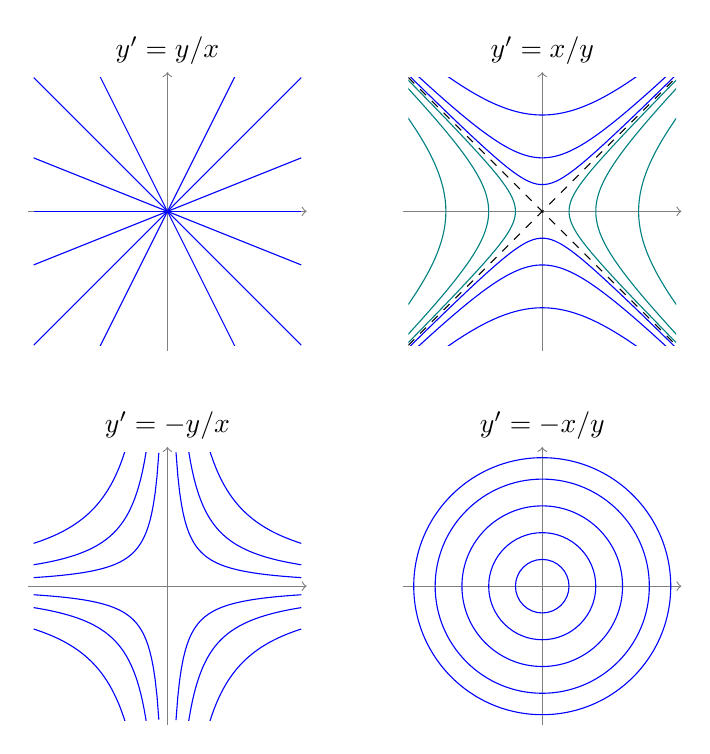
\begin{tikzpicture}[scale=.68]
\foreach \pos/\lab in {0/{y'=y/x},7/{y'=x/y}}{
\begin{scope}[xshift=\pos cm]
\draw[->,gray](-2.6,0)--(2.6,0);\draw[->,gray](0,-2.6)--(0,2.6);
\node at(0,3){$\lab$};
\end{scope}}
\begin{scope}\clip(-2.5,-2.5)rectangle(2.5,2.5);
\foreach \m in {-2,-1,-.4,0,.4,1,2}{\draw[blue](-2.5,{-2.5*\m})--(2.5,{2.5*\m});}
\end{scope}
\begin{scope}[xshift=7cm]\clip(-2.5,-2.5)rectangle(2.5,2.5);
\foreach \a in {.5,1,1.8}{\foreach \s in {-1,1}{
\draw[blue,domain=-2.5:2.5,samples=70]plot(\x,{\s*sqrt(\x*\x+\a*\a)});
\draw[teal,domain=-2.5:2.5,samples=70]plot({\s*sqrt(\x*\x+\a*\a)},\x);}}
\draw[dashed](-2.5,-2.5)--(2.5,2.5);\draw[dashed](-2.5,2.5)--(2.5,-2.5);
\end{scope}
\begin{scope}[yshift=-7cm]
\foreach \pos/\lab in {0/{y'=-y/x},7/{y'=-x/y}}{
\begin{scope}[xshift=\pos cm]
\draw[->,gray](-2.6,0)--(2.6,0);\draw[->,gray](0,-2.6)--(0,2.6);
\node at(0,3){$\lab$};\end{scope}}
\begin{scope}\clip(-2.5,-2.5)rectangle(2.5,2.5);
\foreach \c in {-.4,-1,-2,.4,1,2}{
\draw[blue,domain=.16:2.5,samples=70]plot(\x,{\c/\x});
\draw[blue,domain=-2.5:-.16,samples=70]plot(\x,{\c/\x});}
\end{scope}
\begin{scope}[xshift=7cm]\foreach \r in {.5,1,1.5,2,2.4}{\draw[blue](0,0)circle(\r);}\end{scope}
\end{scope}
\end{tikzpicture}
\end{center}
\textbf{Problem 2.6/1.} Rays, hyperbolas, rectangular hyperbolas, and circles. In the second and fourth panels the points on $y=0$ are outside the displayed equation's domain; in the first and third panels $x=0$ is excluded. The plots show the geometric completions to make their shapes visible.

\begin{center}
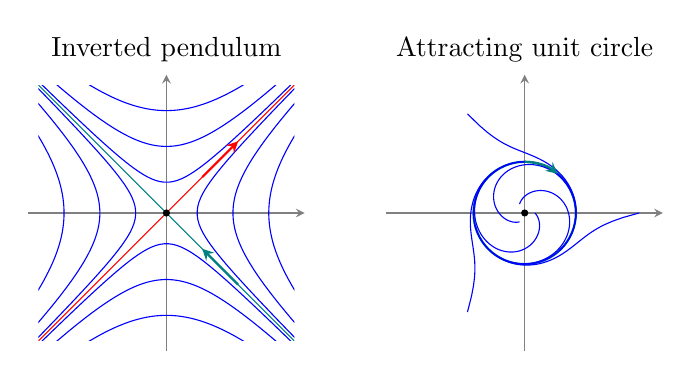
\begin{tikzpicture}[scale=.65,>=stealth]
\begin{scope}
\draw[->,gray](-2.7,0)--(2.7,0);\draw[->,gray](0,-2.7)--(0,2.7);
\node at (0,3.2){Inverted pendulum};
\begin{scope}\clip(-2.5,-2.5)rectangle(2.5,2.5);
\foreach \a in {.6,1.3,2}{\foreach \s in {-1,1}{
\draw[blue,domain=-2.5:2.5,samples=60]plot(\x,{\s*sqrt(\x*\x+\a*\a)});
\draw[blue,domain=-2.5:2.5,samples=60]plot({\s*sqrt(\x*\x+\a*\a)},\x);}}
\draw[teal](-2.5,2.5)--(2.5,-2.5);\draw[red](-2.5,-2.5)--(2.5,2.5);
\draw[->,thick,teal](1.4,-1.4)--(.7,-.7);\draw[->,thick,red](.7,.7)--(1.4,1.4);
\end{scope}\fill(0,0)circle(2pt);
\end{scope}
\begin{scope}[xshift=7cm]
\draw[->,gray](-2.7,0)--(2.7,0);\draw[->,gray](0,-2.7)--(0,2.7);
\node at(0,3.2){Attracting unit circle};
\draw[thick,teal](0,0)circle(1);\fill(0,0)circle(2pt);
\foreach \a in {0,120,240}{
\draw[blue,domain=0:5,samples=110]plot({cos(\a-\x*180/pi)/sqrt(1+24*exp(-2*\x))},{sin(\a-\x*180/pi)/sqrt(1+24*exp(-2*\x))});
\draw[blue,domain=0:5,samples=110]plot({cos(\a-\x*180/pi)/sqrt(1-.8*exp(-2*\x))},{sin(\a-\x*180/pi)/sqrt(1-.8*exp(-2*\x))});}
\draw[->,thick,teal](0,1)arc(90:50:1);
\end{scope}
\end{tikzpicture}
\end{center}
\textbf{Problems 2.5/5 and 5.3/2.} The saddle has a stable diagonal (teal) and an unstable diagonal (red); the second portrait has clockwise spirals approaching the unit circle.

\clearpage
\section*{Review guide and coverage}
\addcontentsline{toc}{section}{Review guide and coverage}
The main logical distinctions to check while reading are: a phase curve versus an integral curve; an invariant level set versus a single maximal orbit; preservation of directions versus preservation of velocity; local solvability versus a complete flow; and a formula obtained by division versus all solutions of the original equation.

\begin{center}\begin{tabular}{llr}\toprule
Book section & Subsections containing numbered problems & Number\\\midrule
$\S1$ & 2, 6, 7, 8, 13, 14, 15, 16, 18 & 17\\
$\S2$ & 1, 3, 5, 6, 7 & 19\\
$\S3$ & 2, 4, 5 & 5\\
$\S4$ & 1, 3, 4 & 21\\
$\S5$ & 1, 2, 3, 4, 5 & 22\\
$\S6$ & 1, 2, 3, 4, 5, 6 & 24\\\midrule
Total & Explicitly numbered problems & 108\\\bottomrule
\end{tabular}\end{center}
The counts include problems for which the textbook already gives a solution. Embedded questions about rigid-body dimension, the dimension of a linear solution space, Floquet bounds, delta sequences, affine period maps, symmetry groups, and distributional Laplacians are also addressed. Subsections with no numbered exercises do not receive artificial problem numbers.

\paragraph{Suggested first review.}
Check $1.7/1$ (the projective-line wording), $1.18/3$--$4$ (quotient and linking), $2.3/1$ (domain at the limiting point), $2.7/2$ (two-sided logarithmic estimates), $5.2/2$ (expressing the pushforward at its image point), $5.4/4$--$5$ (global straightening), and $5.5/3$ (smooth gluing of scalar conjugacies). These are the places where a short answer most readily hides an assumption.

\paragraph{Source.}
Vladimir I. Arnold, \emph{Ordinary Differential Equations}, third edition, translated by Roger Cooke, Springer-Verlag, 1992, Chapter 1, pp.~13--88. Prepared against the scanned copy in the user's library. These notes are an independent worked companion, not an official solution manual.
\end{document}



